Binære tellere gir et binært tall på output som øker med én for hver gang
inngangsklokken tikker.
\\\\
Ved å bruke master/slave flip-flops koblet i serie hvor Q er koblet til neste
sin klokke.
Alle inngangene, J og Q, er satt til høy, slik at hver gang klokka tikke endres
Q og $\overline{Q}$ til det motsatte.
\begin{figure}[H]
  \caption{4bit binærteller.}
  \centering
  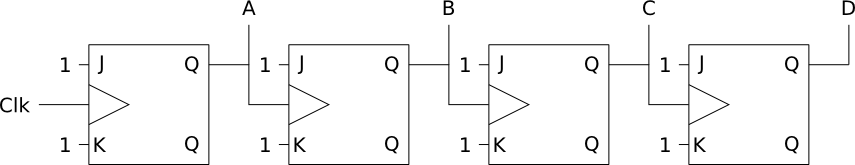
\includegraphics[width=\textwidth]{./img/biteller}
\end{figure}
Output A, B, C og D er little endian.
Det vil si at den minst betydningsfulle biten kommer først.
Dvs $A=2^0$, $B=2^1$ osv.
\\\\
Når klokka tikker, veksler A fra av og på.
Når A tikker, veksler B fra av og på, osv.
Resultatet blir en teller.
\begin{figure}[H]
  \caption{Binærteller output}
  \centering
  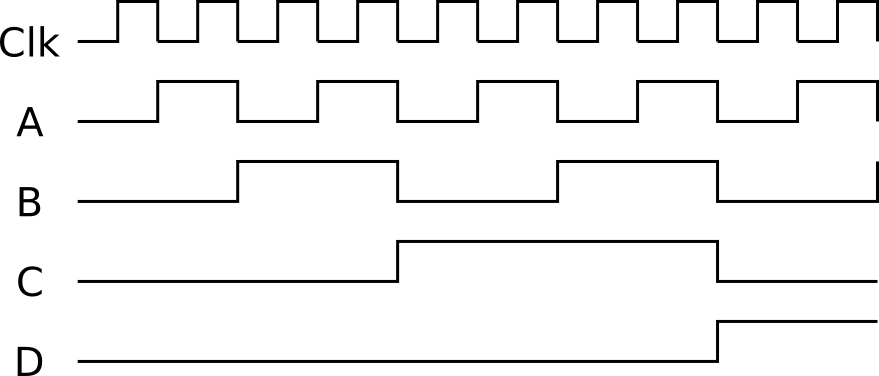
\includegraphics[width=\textwidth]{./img/biteller-output}
\end{figure}
Hvis du ser på output ser du at den teller oppover 0000, 1000, 0100, 1100 osv.
